\chapter{Einleitung}

Im Jahr 2022 erregte OpenAI Aufsehen mit ihrem browserbasierten ChatGPT (Generative Pre-trained Transformer) \cite{2023arXiv230308774O}. In nur fünf Tagen erreichte ChatGPT eine Million Nutzer*innen \cite{doit_software_chatgpt_2025} und ist aus dem Alltag vieler Menschen nicht mehr wegzudenken.
Die GPT-KI (Künstliche Intelligenz) von OpenAI gehört zur Familie der LLMs oder auch Multimodal Large Language Models (MLLMs). MLLMs können neben Text weitere Medien wie zum Beispiel Bilder, Audio und Video verarbeiten.
LLMs von anderen Anbietern wie Googles Gemini \cite{2023arXiv231211805G} und DeepSeek \cite{2025arXiv250112948D} haben mit vergleichbare Qualität und ähnliche Fähigkeiten wie OpenAIs GPT-Modelle.

Die GPT-Modelle von OpenAI und anderen Anbietern wie Googles Gemini \cite{2024arXiv240305530G} sind meistens nur über eine API (Programmierschnittstelle) gegen Entgelt verfügbar.
Open-Source-Modelle wie DeepSeek \cite{2025arXiv250112948D} oder Metas LLAMA \cite{2023arXiv230709288T} erfreuen sich immer größerer Beliebtheit, da sie gratis auf der eigenen Hardware ausgeführt werden können.

Im Oktober 2023 kam der Verfasser dieser Arbeit erstmalig mit RAG in Kontakt; damals war die Idee, mit Hilfe eines LLMs Fragen über mehrere firmeninterne Informationsquellen zu beantworten.
Bei einem Hackathon gelang es dem Team des Verfassers, einen Prototypen (im Folgenden \enquote{KID-System} genannt) zu entwickeln, der mit einem gewissen Erfolg Fragen zu firmeninternen Themen beantworten konnte.

Einer der Schritte während der Entwicklung war das ständige Testen der neuesten Änderungen. Dadurch konnten die Funktionsfähigkeit überwacht und eventuell schlechte Ergebnisse dokumentiert werden.
Diese zeitintensive Aufgabe kostete wertvolle Zeit, die das Team lieber in die Entwicklung investiert hätte.
Gerne hätten wir unterschiedliche Prompts innerhalb unseres KID-Systems getestet oder eine automatische Überprüfung unserer neuesten Änderungen genutzt.

\begin{table}[h!]
    \centering
    \caption[Vergleich der RAG-Evaluierungswerkzeuge]{Vergleich der Open Source RAG-Evaluierungswerkzeuge}
    \label{tab:rag_eval_comparison}
    \begin{tabular}{|l|c|p{0.5\linewidth}|}
        \hline
        \textbf{Werkzeug} & \textbf{GitHub Sterne} & \textbf{Schlüsselwörter} \\
        \hline
        Giskard & 4.7k & KI/LLM/RAG-Evaluierung, Performance, Bias, Sicherheit, Sicherheitslücken-Identifizierung \\
        \hline
        Opik & 10.4k & LLM/RAG/Agenten-Workflows, Debugging, Evaluierung, Monitoring, Tracing \\
        \hline
        Ragas & 9.7k & RAG-spezifische Evaluierung, \textbf{Automatische Testdaten}, Objektive Metriken \\
        \hline
    \end{tabular}
\end{table}

Mittlerweile gibt es viele Arten, LLMs zu bewerten und ein reger Wettbewerb ist um die vielen Bewertungen entstanden.
RAGAS~\cite{es-etal-2024-ragas} wurden entwickelt, um das oben geschilderte Probleme des ständigen Testesns zu lösen.
Es hat zudem das Alleinstellungsmerkmal, dass man weder eigene Fragen noch die generierten Fragen selbst beantworten muss.
Sowohl die Generierung eines Fragenkatalogs (Testsets) als auch die Beantwortung der Fragen, um eine Musterlösung zu erstellen, nimmt RAGAS mithilfe von LLMs vor.
Mithilfe dieses Testsets und von RAGAS eigens entwickelter Metriken, welche die wichtigsten Funktionen eines RAGs abdecken, kann eine Bewertung des Systems vorgenommen werden.

Damit benutzt RAGAS selber LLMs, um das durch LLMs entstandene System zu testen.
Dies spart menschliche Ressourcen, welche zeit- und kostenintensiv sind.
Wie gut LLMs für diese Aufgabe geeignet sind, ist jedoch, auch aufgrund ihrer Halluzinationen, fraglich.
Ragas wurde für diese Arbeit ausgewählt, da es das einzige Tool ist, das alle Komponenten hat, um ein RAG spezifisches System zu testen.
Die anderen Tools, wie Giskard und Opik bieten auch die Möglichkeit, LLMs zu bewerten, der Schritt der Fragen Generierung und der Musterlösung fehlt jedoch.
Um zu verstehen, wie RAGAS arbeitet, werden zunächst die grundlegenden Funktionsweisen von Sprachmodellen erläutert.

\section{Wie funktioniert ein LLM}
Die meisten LLMs heutzutage sind sogenannte Transformer, daher kommt auch das T in GPT. Transformer sind Neuronale-Netzwerk-Modelle, die auf dem Aufmerksamkeits-Mechanismus basieren.
Das Konzept der Aufmerksamkeit wurde im Paper \enquote{Attention Is All You Need} \cite{2017arXiv170603762V} vorgestellt; es ist einer der fundamentalen Bausteine für die heutigen LLMs.
LLMs setzen sich aus vier Schritten zusammen:
\begin{enumerate}
    \item Tokenisierung (Tokenizer)
    \item Einbettung (Embedding)
    \item Berechnung der Wahrscheinlichkeit des nächsten Tokens (Vorhersage)
    \item Strategien zur Auswahl der Ausgabe (manchmal auch Dekodierung genannt).
\end{enumerate}

\enquote{Token sind Wörter, Zeichensätze oder Kombinationen aus Wörtern und Interpunktionszeichen, die von großen Sprachmodellen generiert werden, wenn sie Text zerlegen.}~\cite{microsoft_dotnet_ai_tokens_2025}
Die Aufgabe des Verwandelns der Eingabe in Tokens übernimmt der Tokenizer.

Damit ein Neuronales Netzwerk mit Tokens rechnen kann, müssen diese in Vektoren umgewandelt werden.
Ein Umwandeln in einfache Zahlen reicht hier nicht, da die Fähigkeit benötigt wird, semantische Ähnlichkeiten zu modellieren.
Das Umwandeln ist mithilfe von Embeddings möglich.
Häufig sind Embeddings neuronale Netze, die mit großen Mengen an Texten trainiert wurden, um Wörtern eine Position im höherdimensionalen Raum zu geben.
Diese Position soll die semantische Bedeutung der Wörter beibehalten.

In Abbildung~\ref{fig:sentence_to_embedding} ist ein Beispiel für die Umwandlung eines Satzes in Vektoren zu sehen.
Die Abbildung vereinfacht den Tokenisierungs- und Embedding-Prozess, da Tokens in der Realität nicht immer so klar voneinander getrennt sind und die Vektoren meistens mehrere tausend Dimensionen haben.

\begin{figure}[h!]
    \centering
    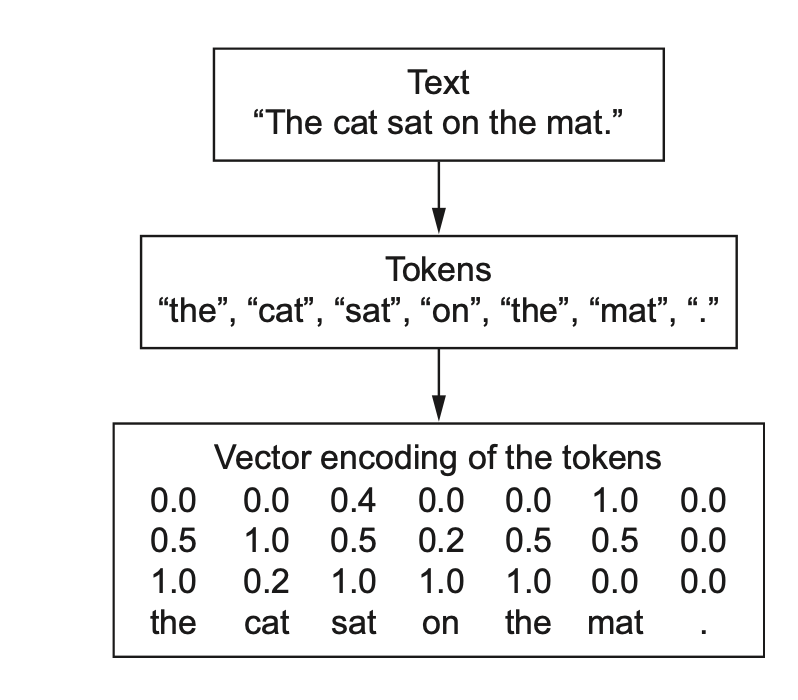
\includegraphics[width=0.4\textwidth]{images/sentence_to_embedding}
    \caption[Embedding Beispiel]{Beispiel für ein Embedding von einem Satz zu Vektoren.}
    \label{fig:sentence_to_embedding}
\end{figure}

Die Vektoren können jetzt in ein Neuronales Netzwerk, das meistens die Transformer-Architektur verwendet, gefüttert werden.
Das Ergebnis besteht aus den Wahrscheinlichkeiten für alle der möglichen nächsten Token.

Im letzten Schritt muss ausgewählt werden, welcher Token genutzt werden soll.
Würde hier immer nur der wahrscheinlichste Token gewählt, würde man nur Texte generieren, die das LLM während des Trainings bekommen hat.
Um einen neuen Text zu generieren werden also zufällig weniger wahrscheinliche Tokens ausgewählt.
Dieser Prozess führt zu dem, was als Halluzinationen bekannt ist.
Es ist ein fester Bestandteil der LLM-Architektur~\cite{fraunhofer_iese2025}.

Mit dem Wissen, wie LLMs funktionieren, kann nun betrachtet werden, wie RAGs funktionieren, wie LLMs mit RAGs kombiniert werden und welche Vorteile RAGs haben.

\section{Funktionsweise von RAGs}

Bei einem Rag kommt das Wissen für die Antwort nicht nur aus dem LLM selbst sondern auch aus angebundenen Quellen.
Diese angebundenen Quellen können Dokumentensammlungen, Datenbanken, Wissensgraphen (Knowledge Graph) oder andere Suchquellen wie eine Internetsuche sein~\cite{honroth2024retrieval}.

\begin{figure}[ht!]
    \centering
    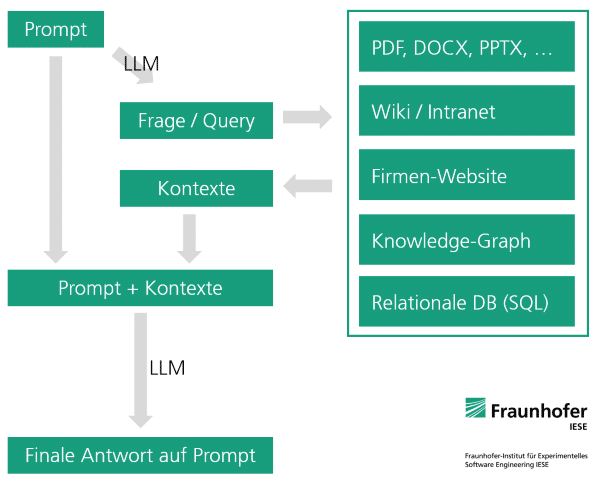
\includegraphics[width=0.8\textwidth]{retrieval_augmented_generation_RAG_600px.png}
    \caption[Struktur eines RAGs]{Struktur eines RAGs, Quelle: \cite{honroth2024retrieval}}
    \label{fig:Rag_Structure}
\end{figure}

Die Abbildung~\ref{fig:Rag_Structure} zeigt den Ablauf für eine Anfrage an ein RAG.
\begin{enumerate}
    \item Im ersten Schritt wird ein Prompt an das LLM gesendet.
    Dieser Prompt besteht aus der Frage des Nutzers, aber auch weiteren Details, wie einer Persona, deren Perspektive das LLM einnehmen soll.
    \item Das LLM kann dann mittels dieses Prompts eine Anfrage generieren, um für diesen Prompt relevante Dokumente zu suchen.
    \item Diese Anfrage gibt dann im optimalen Fall die benötigten Dokumente für die Beantwortung des Prompts zurück.
    Der Schritt des Abfragens relevanter Dokumente wird Retrival genannt.
    Die gefundenen Dokumente werden Kontext genannt.
    \item Der Original Prompt zusammen mit dem abgefragten Kontext wird nun einem LLM zur Verfügung gestellt, um den kontextabhängigen Prompt zu beantworten.
\end{enumerate}
\subsection{Vorteile von RAGs}
Bei der Wissensabfrage durch LLMs zeigen sich unter anderem folgende Schwachstellen:
\begin{description}
    \item [\textbf{Aktualität:}] LLMs kennen nur die verwendeten Trainingsdaten. Es fehl also häufig wissen der letzten Jahre.
    \item [\textbf{Unbalancierte Trainingsdaten:}] Im Trainingsset für die LLMs selten vorkommendes Wissen können LLMs schlecht lernen. \cite{gao2023rtre,2022arXiv221108411K}
    \item [\textbf{Vertraulichkeit:}]Nicht öffentliche Dokumente sind nicht im Trainingsset und daher können LLMs keine Fragen zu nicht öffentlichen Daten beantworten.
\end{description}

Die Nutzung eines RAGs ist eine von drei häufig verwendeten Möglichkeiten, um ein LLM zu verbessern.
Die anderen beiden Möglichkeiten sind Finetuning und die Verwendung eines LLMs mit einem großen Kontextfenster.
Das Finetuning beschreibt das weitere Trainieren eines Modells mit weitere Trainingsdaten.
Die Größe des Kontextfensters beschreibt die Menge an Text, gemessen in Tokens, die das LLM gleichzeitig berücksichtigen kann.
RAGs haben gegenüber dem Finetuning und der Nutzung eines LLMs mit großem Kontextfenster entscheidende Vorteile.\\
ChatGPT-4.1 erreicht inzwischen ein Kontext Window Größe von 1,047,576 Tokens, bei GPT-3.5-Turbo sind es 16,385~\cite{openai_gpt_4_vision}.
Gemini unterstützt ebenfalls bis zu 1 Million Tokens, wobei Google, der Besitzer von Gemini, angibt, dass sie erfolgreich 10 Millionen Token Context Windows getestet haben \cite{google_gemini_next_generation_model}.

\subsection{Faktoren für den Einsatz von RAGs}
Es gibt einige Faktoren, welche die Entscheidung beeinflussen können, ob ein RAG besser für den betrieblichen Ablauf geeignet ist.
Dazu gehören z. B. die Kompetenz der Betreiber des RAGs, die Art der Daten und die finanziellen Möglichkeiten des Unternehmens.


\subsubsection{Kompetenz des Betreibers}
Für das Finetuning von LLMs ist technisches Wissen notwendig, um die Themen Natural Language Processing (NLP), Deep Learning, Modellkonfiguration, Datenaufbereitung und Evaluierung anzuwenden.
Der gesamte Prozess des Finetunings ist technisch anspruchsvoll, erfordert das Kuratieren der neuen Trainingsdaten und ist zudem durch die benötigte Hardware teuer.
Zudem ist das betreiben der Hardware teuer da sie einen hohen Stromverbrauch hat.

Das Benutzen eines LLMs benötigt die geringste Informatische Kompetenz des Anwender, da hier das LLM unverändert bleibt.
Hier werden einfach die Daten inklusive der Frage an das LLM gesendet.
Entscheidend ist allerdings das Erstellen zielführender Prompts, dies benötigt Erfahrung.

Während das LLM in einem RAG auch unverändert bleibt, wird es in ein System mit mehreren Komponenten eingebunden.
Hier ist ein allgemeines Verständnis von LLMs und effektiven Methoden für den Retrieval Teil des RAGs notwendig.
Zudem müssen hier manuell für jedes Dateiformat (E-Mail, PDF etc.) Anbindungen erstellt werden. Sollte ein seltener oder proprietärer Datentyp verwendet werden, muss hier eventuell eigens eine Anbindung entwickelt werden.
\subsubsection{Aktualisierung der Datenbasis}
Sollten die Daten dynamisch sein, wie E-Mails, ist das RAG vermutlich die vorzuziehende Lösung. Dies liegt an den Eigenschaften der schnellen und kontinuierlichen Aktualisierung der Daten.
Wie oben erläutert, kann es jedoch sein, dass es schlechte oder keine Unterstützung von selten verwendeten Dateiformaten gibt.

Der Prozess des Finetunings erstellt hingegen eine Momentaufnahme, die ein erneutes Training erfordert.
Beim Finetuning ist es möglich, dass das Modell Muster erkennt und firmeneigene Begriffe verstehen kann. Dies ist ein deutlicher Vorteil gegenüber dem RAG und dem nutzen eines LLMs mit großem Context Window.


\subsubsection{Budget}
Das Finetuning erfordert über einen langen Zeitraum teure Rechenzeit auf Hochleistungs-Graphical-Processing-Units (Hochleistungs-GPUs).
Dabei handelt es sich um spezialisierte Grafikprozessoren, deren Architektur auf die massive parallele Verarbeitung von Daten optimiert ist, was sie für die rechenintensiven Operationen des Machine Learnings, insbesondere neuronale Netze, unerlässlich macht.
Zudem ist die Qualität der Daten entscheidend; ohne das vorherige Filtern der Daten durch Menschen ist dieser Prozess aktuell nicht möglich. Sollten sich die Daten als unzureichend erweisen, ist die gesamte Rechenzeit verschwendet.
Das RAG verursacht dagegen zusätzliche Kosten durch das Speichern der Daten in einer Vektordatenbank.
Die wohl kostenintensivste Methode ist die Nutzung eines LLMs mit einem großen Kontextfenster.


\section{Objektive Beurteilung von RAGs}
Je mehr Daten einem RAG zur Verfügung stehen, desto aufwendiger ist es, die Qualität des RAGs zu beurteilen.
Eine Beurteilung durch Menschen müsste bei Anpassungen am RAG oder Änderungen an den Daten neu durchgeführt werden.

Tools wie RAGAS, die bereits eine automatisierte Bewertung implementieren, nutzten bei diesem Prozess unter anderem LLMs.
Diese Tools generieren aus den ihnen gegebenen Daten Fragebögen, die zu einer Frage eine beispielhafte Antwort und die genutzten Stellen aus den vorher gegebenen Dokumenten beinhalten.
Sollten nach diesem automatisierten Test die gewünschten Ergebnisse nicht erreicht werden, kann beispielsweise die Veröffentlichung blockiert werden.

Sowohl menschliche Bewertungen als auch je nach Vorgaben die eventuell subjektive Bewertung durch LLMs sind nicht objektiv.
Anhand mehrerer Techniken kann versucht werden, die Bewertung mithilfe von LLMs zu objektivieren. Die Metriken, welche RAGAS nutzt, versuchen z.B. die Anzahl der genannten Fakten aus den Antworten zu extrahieren, um so mit Zahlen arbeiten zu können.

\section{Softwaretechnische Fragestellungen}

In dem Artikel \textit{RAG in der Praxis – Generierung synthetischer Testdatensätze} untersucht Panic~\cite{pixion2024rag} die Testset-Generierung mithilfe von RAGAS. Es treten bei 17 \% der generierten Fragen Fehler beim Generieren der Testfragen auf.
Dies hat vielfältige Gründe, die von nicht verwertbaren Antworten des LLMs bis zu Verbindungsproblemen oder dem Erreichen des Limits der maximalen Anfragen an APIs reichen.

Auch bei der Bewertung von Antworten können sich ungewollte und bisher noch ungeahnte Biases einschleichen. In dem Paper \enquote{Large Language Models are not Fair Evaluators}~\cite{wang-etal-2024-large-language-models-fair} von Wang et al. wird gezeigt, dass, wenn ein LLM eine von zwei gegebenen Antworten aussuchen müsste, die erste bevorzugt wurde, selbst wenn die gleiche Frage mit einer anderen Reihenfolge gestellt wurde.
RAGAS vergleicht keine Antworten miteinander, und daher ist dieser Bias kein direktes Problem für die verwendeten Metriken. Was jedoch einen Einfluss auf die Bewertung von Antworten haben kann, ist der Bias zu gewissen Nummern.
Wie in~\cite{2024arXiv241203605S} von Shaikh et al. beschrieben, bevorzugen LLMs bei der Bewertung lieber Zahlen, welche Vielfache von 5 und 10 sind.

Auch die allgemeine stochastische Natur von LLMs spielt eine Rolle, da bei der gleichen Anfrage unterschiedliche Antworten und somit auch Bewertungen zurückgegeben werden.
Wie groß diese Abweichungen sind, wird in Abschnitt~\ref{subsec:zuverlassigkeit-von-metriken} kurz untersucht.

Wie in dem Paper \enquote{Gemini 1.5: Unlocking multimodal understanding across millions of tokens of context} vom Gemini Team \cite{gemini2024v15} beschrieben, stellt Gemini 1.5 einen bedeutenden Fortschritt in der multimodalen Verarbeitung großer Kontextfenster dar. Das wirft auch die Frage auf, ob RAGs nicht irrelevant sein könnten und durch LLMs mit großen Kontextfenstern abgelöst werden.
Es gibt einige Gründe, die dagegen sprechen: LLMs mit größeren Kontextfenstern werden immer langsamer und teurer; die genauen Kosten sind abzuwarten. Jedes Mal alle Daten in den Kontext zu laden, besonders wenn dies über das Internet geschieht, ist eine weitere Hürde. LLMs fällt es auch schwer, bei zu vielen Informationen noch die relevanten zu finden, was zu schlechteren Antworten führen kann.
Diese Faktoren lassen darauf schließen, dass RAGs, die nicht nur eine einfache Suche nutzen, noch länger relevant bleiben.

Inzwischen werden spezielle LLMs wie Pleias-RAG~\cite{huggingface_pleias_rag_1b} entwickelt.
Diese wurde mittels Finetuning verbessert, um Speziell Aufgaben wie das Suchen und das Zusammenfassen von Dokumenten selbst mit weniger Parametern gut zu können.

% Pitfalls in LLM Assisted Evaluation https://medium.aiplanet.com/evaluate-rag-pipeline-using-ragas-fbdd8dd466c1

\section{Rechtliche Fragestellungen}
\label{sec:rechtliche-fragestellungen}

Am 01.08.2024 trat die \\
\enquote{\textit{VERORDNUNG (EU) 2024/1689 DES EUROPÄISCHEN PARLAMENTS UND DES RATES vom 13. Juni 2024 zur Festlegung harmonisierter Vorschriften für künstliche Intelligenz und zur Änderung der Verordnungen (EG) Nr. 300/2008, (EU) Nr. 167/2013, (EU) Nr. 168/2013, (EU) 2018/858, (EU) 2018/1139 und (EU) 2019/2144 sowie der Richtlinien 2014/90/EU, (EU) 2016/797 und (EU) 2020/1828 (Verordnung über künstliche Intelligenz)}} (KI-VO)~\cite{european_commission_ai_act}\\
in Kraft.
Die Verordnung setzt Regelungen und Maßstäbe für die Verwendung von KI.
RAGs sind gemäß Artikel 3 Nr. 1 in Verbindung mit Artikel 51 KI-VO KI-Systeme~\cite{Martini2024KIVO} und fallen damit in den Anwendungsbereich der KI-VO.
Bei der Nutzung oder Bereitstellung von LLMs muss die KI-VO berücksichtigt werden.
Die Nutzer*innen der RAGs müssen sich der aus der KI-VO ergebenden Pflichten bewusst sein.\\
Ebenso gilt es, bei Anbindung firmeninterner Dokumente die\\
\enquote{\textit{Verordnung (EU) 2016/679 des Europäischen Parlaments und des Rates vom 27. April 2016 zum Schutz natürlicher Personen bei der Verarbeitung personenbezogener Daten, zum freien Datenverkehr und zur Aufhebung der Richtlinie 95/46/EG (Datenschutz-Grundverordnung)}} (DS-GVO) zu beachten.
Die DS-GVO regelt den Umgang mit personenbezogenen Daten, die in solchen firmeninternen Dokumenten enthalten sein könnten.
